\section{System Architecture}
\label{sec:architecture}

StretchBot is structured around a four-stage pipeline: Perception, Reasoning, Action Execution, and Planning \& Adaptation. Each stage transforms information into increasingly higher-level representations, enabling the robot to adapt its behavior in real time. Figure~\ref{fig:overall_pipeline} summarizes this closed control loop and the direction of information flow.

\begin{figure*}[t]
\centering
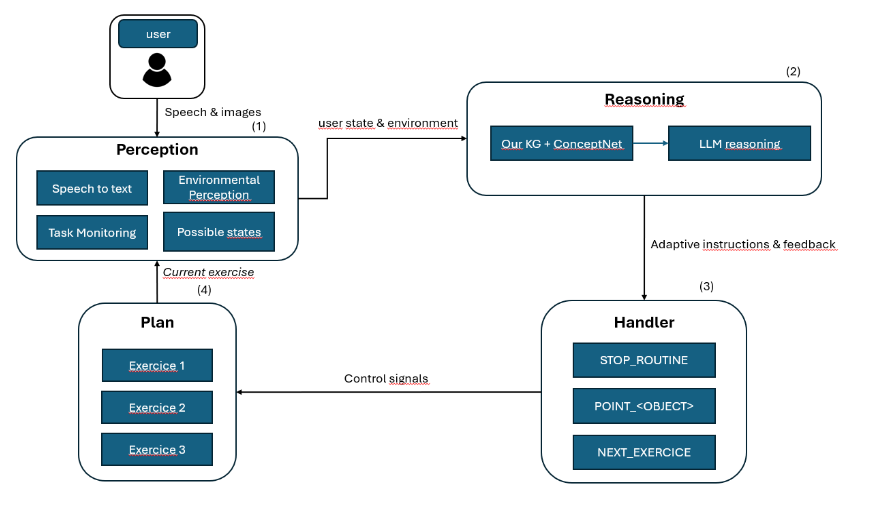
\includegraphics[width=0.92\textwidth]{../images/figure1_pipeline.png}
\caption{Overall StretchBot pipeline organized into four stages: Perception, Reasoning, Action Execution (Handler), and Planning \& Adaptation. The numbered markers indicate the main flow steps discussed in the text.}
\label{fig:overall_pipeline}
\end{figure*}

The numbered markers in Figure~\ref{fig:overall_pipeline} correspond to the operational sequence used in our implementation. Marker \textbf{(1)} denotes the multimodal input transfer from the user to the \textit{Perception} block (speech and image streams). Marker \textbf{(2)} denotes the transition from perceived user/environment state to the \textit{Reasoning} block, where KG + ConceptNet context is combined with LLM reasoning. Marker \textbf{(3)} denotes the delivery of adaptive instructions and feedback from \textit{Reasoning} to the \textit{Handler} (execution interface using actions such as \texttt{NEXT\_EXERCISE}, \texttt{POINT\_<OBJECT>}, and \texttt{STOP\_ROUTINE}). Marker \textbf{(4)} denotes the control feedback from the Handler to the \textit{Plan} block, which updates the current exercise stage and closes the adaptation loop.

\subsection{Perception Module}

In Figure~\ref{fig:overall_pipeline}, this module is the left block and corresponds to the first stage of the loop. The perception module provides the adaptive system with a continuous and multimodal understanding of both the user's state and the environment. It integrates four complementary components:

\subsubsection{Object Detection}
Visual scene analysis is performed using YOLOv8 \cite{ref18}, applied to the live RGB feed from the robot's camera. The system retrieves the complete list of all detected objects in the scene and sends this list to the reasoning module, ensuring that every recognized element is available for potential reasoning or adaptation.

\subsubsection{Multimodal Emotion Recognition}
The user's emotional state is inferred through the fusion of three independent detection channels:
\begin{itemize}
\item \textit{Voice emotion recognition}—using a HuggingFace Transformers pipeline \cite{ref19} on speech segments captured by the microphone.
\item \textit{Facial emotion recognition}—using DeepFace \cite{ref20} applied to the video stream.
\item \textit{Text-based emotion recognition}—using a lightweight HuggingFace model \cite{ref19} on transcribed speech.
\end{itemize}

A dedicated fusion module performs weighted fusion and majority voting to produce a single aggregated emotional state, which is then summarized in natural language for the LLM.

\subsubsection{Task Monitoring}
Task monitoring verifies, in real time, that the user is correctly performing each stretching exercise and holding the required pose for the prescribed duration. It relies on \textbf{MediaPipe Pose} \cite{ref21}, a lightweight skeleton-estimation library that infers the positions of 33 body landmarks (shoulders, elbows, wrists, hips, ankles, etc.) from a single RGB frame at 30\,Hz.

\paragraph{Per-exercise pose criteria.}
Each exercise is evaluated by a dedicated geometric check applied to the MediaPipe landmark coordinates:

\begin{itemize}
\item \textit{Arms above the head.} The system checks that both wrists and both elbows have a $y$-coordinate strictly lower than the nose landmark ($y_\text{wrist} < y_\text{nose}$ and $y_\text{elbow} < y_\text{nose}$, where lower $y$ means higher in the frame), and that the horizontal distance between the two wrists is below a threshold $w_\text{max} = 0.3$ (in normalised image coordinates), ensuring the arms are raised and approximately centred above the head.

\item \textit{Touch-your-toes.} The system computes the Euclidean distance in normalised image coordinates between each wrist landmark and each ankle landmark:
\begin{equation}
d_{ij} = \sqrt{(x_{\text{wrist},i} - x_{\text{ankle},j})^2 + (y_{\text{wrist},i} - y_{\text{ankle},j})^2}\,,
\label{eq:toe_distance}
\end{equation}
and accepts the pose when any $d_{ij} < 0.4$.

\item \textit{Lateral trunk lean (left / right).} The system computes the midpoint of the shoulders $M_s$ and the midpoint of the hips $M_h$, then calculates the signed trunk inclination angle:
\begin{equation}
\alpha = \arctan\!\left(\frac{M_{s,x} - M_{h,x}}{M_{h,y} - M_{s,y}}\right),
\label{eq:trunk_angle}
\end{equation}
where the $y$-axis inversion accounts for OpenCV's top-down coordinate origin. The user is classified as leaning \textit{right} when $\alpha > 15^\circ$ and \textit{left} when $\alpha < -15^\circ$.
\end{itemize}

\paragraph{Hold-duration accumulation and reset.}
At each valid frame the hold timer is incremented by the fixed frame period $\Delta t = 1/30\,\text{s}$, capped at the target duration $T = 5\,\text{s}$. If the user holds an invalid pose for longer than a reset tolerance of $t_\text{reset} = 40\,\text{s}$, the timer is zeroed and corrective spoken feedback is issued via the TTS channel. Once the timer reaches $T$, the task monitor emits a success event that propagates via markers \textbf{(3)} and \textbf{(4)} in Figure~\ref{fig:overall_pipeline}.

For the lateral lean exercise, two independent timers track the left-side and right-side hold durations; both must reach $T = 5\,\text{s}$ before the exercise is marked complete.

All pose checks are purely geometric and frame-local, requiring no additional training data beyond the pre-trained MediaPipe model.

\subsubsection{Speech-to-Text (STT)}
The STT component converts the user's spoken input into text for downstream processing. Vosk \cite{ref22} was initially used due to its lightweight local deployment, with Google Cloud Speech-to-Text \cite{ref23} considered for higher accuracy.

All perception outputs are structured into a unified context package containing the detected objects, the aggregated emotional state, the current task execution status, and the most recent STT transcript. This package operationalizes marker \textbf{(1)} and is transmitted to the reasoning block through marker \textbf{(2)} in Figure~\ref{fig:overall_pipeline}.

\subsection{Reasoning Module}

In Figure~\ref{fig:overall_pipeline}, this module is the upper-right block that receives the perception context through marker \textbf{(2)} and sends actionable output to the handler through marker \textbf{(3)}. The reasoning module serves as the central decision-making component, responsible for determining the robot's next action by combining perception outputs, prior knowledge, and the predefined stretching routine. Its operation follows a hybrid approach: rule-based checks handle explicitly defined conditions, while an LLM provides high-level reasoning, contextual adaptation, and natural-language interaction.

\subsubsection{Context Integration and Knowledge Graph Retrieval}

Each time the user speaks, the reasoning module compiles an updated context package including:
\begin{itemize}
\item the list of objects detected by perception,
\item the aggregated emotional state,
\item the current exercise progress status,
\item the latest speech-to-text transcription.
\end{itemize}

To provide the LLM with meaningful background knowledge, this raw context is enriched with semantic relations retrieved from a Knowledge Graph (KG). A knowledge graph is a structured representation of concepts (nodes) and their relationships (edges), often expressed as triples like (coffee, reduces, fatigue) \cite{ref26}. Unlike unstructured text, a KG enables the system to reason over entities and their connections in a transparent and interpretable way.

\subsubsection{LLM-Based Adaptive Reasoning}

The complete context package is passed to the primary LLM through a structured prompt. The model analyzes this information to decide the most appropriate next step in the stretching session, adapting the style and tone of its response to match the detected emotional state. If relevant objects are available in the scene, the model may refer to them directly in its suggestions.

The LLM adheres to predefined action prefixes in its outputs:
\begin{itemize}
\item \texttt{NEXT\_EXERCISE:} instructs the system to move to the following stretch.
\item \texttt{POINT\_<OBJECT>:} directs the robot to point to a detected object.
\item \texttt{STOP\_ROUTINE:} ends the stretching session.
\end{itemize}

\subsubsection{Response Verification}

Once the primary LLM has generated a response, it is passed to a secondary, smaller LLM acting as a verifier. This verification stage maintains the quality and consistency of interactions by checking the message format, confirming appropriate tone, and ensuring coherence with the current session context. The verified output is then emitted as adaptive instructions and feedback, which corresponds directly to marker \textbf{(3)} in Figure~\ref{fig:overall_pipeline}.

\subsection{Action Execution Module}

This module corresponds to the \textit{Handler} block in Figure~\ref{fig:overall_pipeline}. The action execution module grounds high-level reasoning decisions in concrete robot behavior. It acts as the interface between symbolic instructions and the physical world, ensuring that every action is carried out in a synchronized, safe, and comprehensible manner.

\subsubsection{Command Interpretation}
Each output from the reasoning stage arrives in dual format: a structured action prefix and a natural-language sentence. The action prefix encodes the intended behavior in machine-readable form, while the text provides a human-friendly explanation.

\subsubsection{Physical Execution of Movements}
Once a symbolic command such as \texttt{POINT\_Coffee} has been issued, the system translates it into a fixed Cartesian target pose. The target is passed to MoveIt \cite{ref31}, which computes a feasible joint-space trajectory while avoiding collisions. The trajectory is optimized using cubic spline interpolation \cite{ref32} to ensure smooth and continuous motion.

The final optimized trajectory is executed step by step on the Lynxmotion SES900 arm \cite{ref33}. Once the target pose is reached within tolerance, an ``execution finished'' event is published back to the reasoning module.

\subsubsection{Verbal Feedback and Synchronization}
In parallel with motion control, text-to-speech (TTS) converts the LLM's natural-language output into spoken instructions. The timing of speech and movement is carefully coordinated to enhance clarity and naturalness of the interaction \cite{ref34}. The system supports multiple voices, ranging from simple rule-based synthesis to expressive neural voices capable of conveying emotion \cite{ref35}, reinforcing empathy and engagement.

\subsubsection{Safety Supervision}
A critical aspect of execution is maintaining user safety and hardware integrity. The module integrates a watchdog subsystem that supervises all ongoing actions:
\begin{itemize}
\item Joint limits and velocity clamping prevent excessive extension or unsafe speed.
\item Collision detection monitors the environment for potential collisions.
\item Emergency stop immediately halts execution if anomalies are detected.
\end{itemize}

After execution status is updated, the handler sends control feedback to the planning block, implementing marker \textbf{(4)} in Figure~\ref{fig:overall_pipeline}.

\subsection{Planning and Adaptation Module}

In Figure~\ref{fig:overall_pipeline}, this module is the lower-left \textit{Plan} block. It receives control feedback from the handler via marker \textbf{(4)} and maintains the current exercise state that is fed back into perception for the next cycle. The planning and adaptation module ensures that StretchBot delivers a stretching session that is both structured and responsive.

\subsubsection{Global Routine Structure}
At its core, the system relies on a predefined exercise script composed of a sequence of stretching primitives (e.g., arm stretch, side bend, neck rotation). Each primitive specifies the expected body posture, target hold duration (5 s), and the transition to the next exercise. This script acts as a baseline plan that guarantees coverage and maintains a clear flow.

\subsubsection{Local Adaptations}
On top of this baseline, the system introduces adaptive branching points where the flow can be adjusted depending on the user's state. For example:

\begin{itemize}
\item If the user reports fatigue, the system may suggest a brief pause or recommend a coffee break while maintaining the overall sequence.
\item If the user expresses discomfort with a particular stretch, the system can substitute a gentler alternative or skip to the next exercise.
\item If relevant objects are detected in the environment, the system proactively offers suggestions (e.g., ``I see a bottle of water nearby—would you like a sip?'').
\end{itemize}

These adaptations occur within the framework of the global routine, ensuring that the session remains coherent and goal-directed while accommodating individual preferences and states. Together, markers \textbf{(1)} to \textbf{(4)} therefore describe one complete adaptation cycle that readers can follow in parallel with this section.
